\claude{
\section{Further tests of practical decisions}\label{app:campaign}
\subsection{Self-supervised representation selection}
We train MNIST encoders with SimSiam, BYOL, VICReg, and SimCLR \citep{chen2021simsiam,grill2020byol,bardes2022vicreg,chen2020simclr}. We freeze each encoder and fit a linear classifier to its features from labeled images. On development runs, we choose which log to analyze and whether to rank configurations by increasing or decreasing values of each statistic. We maximize the rank agreement with classifier accuracy. \cx{We rank configurations by decreasing MG on the gradient-norm log.} On evaluation runs, we keep these choices fixed and test classifier accuracy on the same set of images (Table~\ref{tab:ssl-protocol}).

\begin{table}[htbp]
\centering\small
\caption{Protocol for the MNIST representation study.}
\label{tab:ssl-protocol}
\begin{tabularx}{\linewidth}{@{}p{.26\linewidth}X@{}}
\toprule
Component & Setting \\
\midrule
Training settings & 29 configurations. Train for 3,000 \cx{SGD updates} with batches of 128 images and momentum 0.9. \cx{The learning rate rises linearly for 100 updates, then stays fixed. Defaults are learning rate $0.05$, weight decay $10^{-4}$, and medium-strength augmentation.} \\
\cx{SimSiam (13)} & \cx{Use the default and change one setting at a time. Learning rate $0.01$, $0.2$, or $0.5$, weight decay $0.001$, $0.005$, or $0.02$, weak or strong augmentation, no predictor, gradients through both sides of each comparison, 16 projection coordinates, or no projector batch normalization.} \\
\cx{BYOL (4)} & \cx{Use the default and change one setting at a time. Reduce the target averaging coefficient from $0.99$ to $0.9$, remove the predictor, or use strong augmentation.} \\
\cx{VICReg (7)} & \cx{Use learning rate $0.01$ and loss weights $(25,25,1)$ for invariance, variance, and covariance. Separate variants use learning rate $0.05$, variance weight $0$ or $5$, covariance weight $0$ or $10$, or weak augmentation.} \\
\cx{SimCLR (5)} & \cx{Use temperatures $0.1$, $0.5$, and $2$ with medium augmentation, plus $0.2$ with weak or strong augmentation.} \\
\cx{Augmentation settings} & \cx{Entries give translation in pixels, rotation in degrees, scale half-range, erase probability, erase-size factor $b$, Gaussian noise SD, and pixel-drop probability. Weak uses $(2,10,0.05,0,0,0.05,0)$, medium $(4,20,0.15,0.5,0.5,0.10,0.10)$, and strong $(6,30,0.25,0.8,0.7,0.25,0.30)$. For erasing, each half-side is uniform on $[2,2+14b]$ pixels.} \\
Development and evaluation & 2 development and 5 evaluation repeats on the same task \\
Linear classifier & Standardize the encoder features. Fit logistic regression on 5,000 labeled images and test on 5,000 separate images. Inverse regularization strength $C=0.1$, at most 300 solver iterations. \\
Candidate scalar logs & Loss, parameter norm, gradient norm, and encoder and projector norms for one fixed image \\
RankMe & Encoder and projector features from 2,048 images \\
$\alpha$-ReQ & Log--log slope on the first 128 encoder covariance eigenvalues; slope and distance-to-one scores \\
LiDAR & Projector features from 256 images with eight augmentations each; within-image covariance ridge $10^{-4}$ \\
\bottomrule
\end{tabularx}
\end{table}


All scalar methods receive the same candidate logs. Undefined scores rank last. RankMe, $\alpha$-ReQ, and LiDAR use features from many images \citep{garrido2023rankme,agrawal2022alphareq,thilak2024lidar}. In Table~\ref{tab:ssl_campaign}, $h$ denotes the encoder output and $z$ denotes its transformation by the projection network used in training. \cx{For the scaled mean coordinate standard deviation (SD), we normalize each $z$ to unit length, compute the standard deviation of each coordinate across images, and average across coordinates. We multiply this mean by the square root of the number of coordinates.}

\begin{figure}[htbp]
\centering
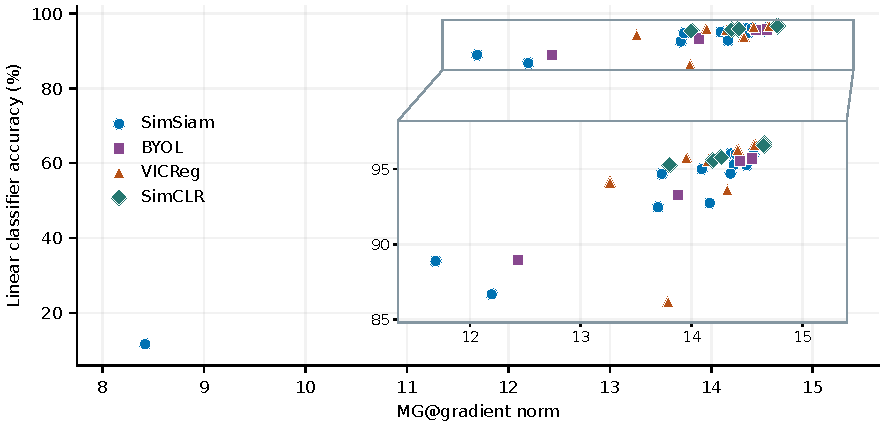
\includegraphics[width=.86\linewidth]{figures/ssl_probe_scatter.pdf}
\caption{MG@gradient norm and test accuracy of a linear classifier fitted to frozen features. Each point averages the evaluation repeats for one configuration.}
\label{fig:ssl-probe-scatter}
\end{figure}

We average rank correlation and accuracy gap over five evaluation repeats. The gap is the best minus the selected accuracy in percentage points. Intervals for $\Delta\rho=\rho_{\rm MG}-\rho_{\rm comparison}$ resample configurations while keeping their initializations together.

\begin{table}[htbp]
\centering\small
\caption{Rank correlation and accuracy gaps for representation selection.}
\label{tab:ssl_campaign}
\begin{tabular}{lrr}
\toprule
Score & \cx{Mean Spearman $\rho$} & Regret (pp) \\
\midrule
MG (gradient norm) & 0.712 & 0.41 \\
Embedding spread & 0.730 & 1.46 \\
Spectral entropy & 0.595 & 1.00 \\
Roughness & 0.599 & 1.20 \\
Delay covariance PR & 0.626 & 1.08 \\
Correlation dimension & 0.594 & 0.75 \\
Recurrence error & 0.474 & 18.13 \\
RankMe ($h$) & 0.321 & 4.00 \\
RankMe ($z$) & 0.522 & 1.46 \\
$\alpha$-ReQ slope & 0.404 & 1.46 \\
LiDAR ($z$) & 0.124 & 85.03 \\
\cx{Random configuration} & --- & 5.47 \\
\bottomrule
\end{tabular}

\end{table}

\Needspace{6\baselineskip}
\subsection{Warning of slingshot loss spikes}
A transformer learning modular addition can show sharp increases in loss called slingshot spikes \citep{thilak2022slingshot}. We test whether a statistic of recent log loss crosses a threshold before a spike. We fix the threshold and direction of change on development runs. To label spike onsets for evaluation, we compare the loss immediately after each step with the earlier loss (Table~\ref{tab:spike-protocol}).

\begin{table}[htbp]
\centering\small
\caption{Protocol for early warning of transformer loss spikes.}
\label{tab:spike-protocol}
\begin{tabularx}{\linewidth}{@{}p{.25\linewidth}X@{}}
\toprule
Component & Setting \\
\midrule
Task & Predict the sum modulo 97 given two operands followed by a delimiter. The training fraction is the share of all operand pairs used for training. \\
Training configurations & \begin{tabular}[t]{@{}rrl@{}}
Learning rate & \cx{AdamW $(\beta_1,\beta_2)$} & Training fraction \\
$10^{-3}$ & \cx{$(0.9,0.98)$} & 30\% \\
$2\cdot10^{-3}$ & \cx{$(0.9,0.98)$} & 30\% \\
$10^{-3}$ & \cx{$(0.9,0.95)$} & 30\% \\
$10^{-3}$ & \cx{$(0.9,0.98)$} & 50\%
\end{tabular} \\
Optimizer and schedule & AdamW with zero weight decay. Each update uses 256 examples. The learning rate rises linearly to its listed value in 100 updates and then stays fixed through update 8,000. \\
Spike onset & The mean log loss over the next 10 updates must exceed the median over the previous 200 by more than one base-10 log unit and more than six times the estimated spread. Spread is 1.4826 times the median absolute deviation of the previous log losses. After an onset, wait 300 updates before labeling another. Nonfinite loss also counts as an onset. \\
Scored warnings & \cx{Score windows from update 1,500 and onsets after it.} A warning counts toward detecting a spike if it occurs within 500 updates before onset. Exclude the onset and the next 500 updates from scoring. Alarms outside all advance warning intervals are false positives (FP). \cx{Skip any such alarm less than 500 updates after the last counted false alarm.} \\
Calibration and evaluation & For each configuration, four runs calibrate the rule and four separate runs evaluate it. Calibration allows at most two false positives per 10,000 scored updates. \\
\bottomrule
\end{tabularx}
\end{table}

\cx{The input in Table~\ref{tab:spikes_campaign} is selected on development runs. We take base-10 logs of loss, gradient norm, and update norm after flooring at $10^{-12}$. Window statistics use the samples before the scoring time. For direct monitoring we use the mean, minimum, or maximum over the latest stride. We test signed levels and signed differences from the median of four or ten older scores, ending one window earlier.}

\cx{Recurrence error minimizes the normalized squared difference over lags of 20--250 samples, using twice the window variance for normalization. Spectral entropy uses the nonzero-frequency periodogram of the centered signal. Recurrence rate, correlation dimension, TwoNN, and delay covariance PR use $E=20$ and unit lag. Recurrence rate counts the fraction of time-separated pairs closer than one tenth of their median distance. Correlation dimension fits the slope of the log fraction of pairs below a radius against the log radius at eight distance quantiles from 0.01 to 0.10~\citep{grassberger1983measuring}. Both pair statistics exclude pairs separated by at most one delay span.}

\cx{We take the maximum attention logit over examples, positions, heads, and layers. For attention entropy, we first average across examples and query positions, then take the minimum across heads and layers. The output log-partition is $\log\sum_c \exp(o_c)$ for class scores $o_c$, averaged over output positions and examples at each step.}

Table~\ref{tab:spikes_campaign} reports counts at the calibrated thresholds and the area under the receiver operating characteristic curve (AUROC). \cx{For AUROC, a scored window is positive if it ends in an advance-warning interval.}

\begin{table}[htbp]
\centering\small
\caption{Advance warnings of transformer loss spikes. \cx{False alarms are per 10,000 scored updates.}}
\label{tab:spikes_campaign}
\begin{tabular}{llrrr}
\toprule
Statistic & \cx{Input} & Detections & \cx{False alarms / 10,000} & AUROC \\
\midrule
Detrended lag-one correlation & \cx{Weight norm} & 23/23 & 2.34 & 0.951 \\
\cx{Minimum loss} & \cx{Loss} & 23/23 & 2.34 & 0.946 \\
Roughness & \cx{Loss} & 23/23 & 2.44 & 0.960 \\
Delay-vector covariance PR & \cx{Loss} & 23/23 & 2.66 & 0.959 \\
Recurrence error & \cx{Loss} & 23/23 & 2.76 & 0.960 \\
Relative detrended standard deviation & \cx{Loss} & 23/23 & 2.76 & 0.931 \\
\cx{Minimum gradient norm} & \cx{Gradient norm} & 22/23 & 2.34 & 0.917 \\
\textbf{MG} & \cx{Loss} & 22/23 & 2.44 & 0.949 \\
Detrended standard deviation & \cx{Loss} & 22/23 & 2.44 & 0.923 \\
Spectral entropy & \cx{Loss} & 21/23 & 2.02 & 0.962 \\
TwoNN dimension estimate & \cx{Loss} & 21/23 & 2.12 & 0.889 \\
\cx{Maximum log-partition} & \cx{Output scores} & 20/23 & 1.91 & 0.827 \\
Recurrence rate & \cx{Gradient norm} & 20/23 & 2.44 & 0.726 \\
MG (lag 4, 50 neighbors) & \cx{Gradient norm} & 20/23 & 2.66 & 0.927 \\
Permutation entropy & \cx{Loss} & 19/23 & 2.23 & 0.881 \\
Trend crossings & \cx{Update norm} & 17/23 & 2.44 & 0.841 \\
Minimum attention entropy & \cx{Attention} & 15/23 & 1.59 & 0.911 \\
\cx{Maximum update norm} & \cx{Update norm} & 15/23 & 2.34 & 0.788 \\
\cx{Minimum weight norm} & \cx{Weight norm} & 14/23 & 3.40 & 0.716 \\
Correlation dimension & \cx{Gradient norm} & 12/23 & 2.44 & 0.882 \\
Maximum attention logit & \cx{Attention} & 4/23 & 1.70 & 0.645 \\
\bottomrule
\end{tabular}

\end{table}

\Needspace{6\baselineskip}
\subsection{Reset rules, schedules, and transfer}
Plasticity is the ability to learn a new task after training on earlier ones. In sequential MNIST, each task changes the pixel order and one set of tasks also adds noise. The rules decide when to reset weights and optimizer state. \cx{The low-activation rule uses the fraction of neurons whose mean absolute activation is small relative to their layer mean \citep{sokar2023dormant}.} We measure accuracy on each batch before its update and average across tasks (Table~\ref{tab:reset-rules}).

\begin{table}[htbp]
\centering\small
\caption{Accuracy on sequential MNIST tasks, across 12 sequences per condition.}
\label{tab:reset-rules}
\begin{tabular}{lrrr}
\toprule
Input condition & MG reset rule & Low-activation reset rule & No resets \\
\midrule
Reordered pixels & 0.873 & 0.880 & 0.845 \\
Reordered pixels and noise & 0.834 & 0.843 & 0.776 \\
\bottomrule
\end{tabular}
\end{table}

\begin{table}[!htbp]
\centering\small
\setlength{\abovecaptionskip}{4pt}
\caption{Additional tests of decisions from scalar logs.}
\label{tab:campaign_scope}
\begin{tabularx}{\linewidth}{@{}>{\raggedright\arraybackslash}p{.30\linewidth}>{\raggedright\arraybackslash}p{.21\linewidth}>{\raggedright\arraybackslash}X@{}}
\toprule
Task & MG result & Comparison \\
\midrule
When to reduce the learning rate on CIFAR-10 & Final accuracy $0.574$ & Fixed late reduction $0.590$, constant rate $0.543$, 24 runs \\
Classifying the number of independent oscillations from game payoffs & Accuracy $0.523$ & Count of fundamental frequencies $0.713$, principal components of the full state about $0.99$, 216 new games. Classes $1$, $2$, and $\ge 3$. \\
Transferring an MNIST detector across data and training settings & $26/87$ detections, $10/58$ false positives & Standard deviation after removing the trend, divided by the window level, gives $85/87$ detections and $9/58$ false positives across ten settings. \\
\bottomrule
\end{tabularx}
\end{table}
}
